\begin{minipage}{.6\linewidth}
	\vspace{-4cm}
	\item No instante mostrado, duas forças atuam sobre a barra fina de \SI{15}{\kilogram} que está presa com pino em $O$. Determine a intensidade da força $F$ e a aceleração angular inicial da barra, de maneira que a reação horizontal que o pino exerce sobre a barra seja \SI{25}{\newton} direcionada para a direita.
\end{minipage}
\begin{minipage}{.4\linewidth}
	\vspace{1cm}
	\begin{flushright}
		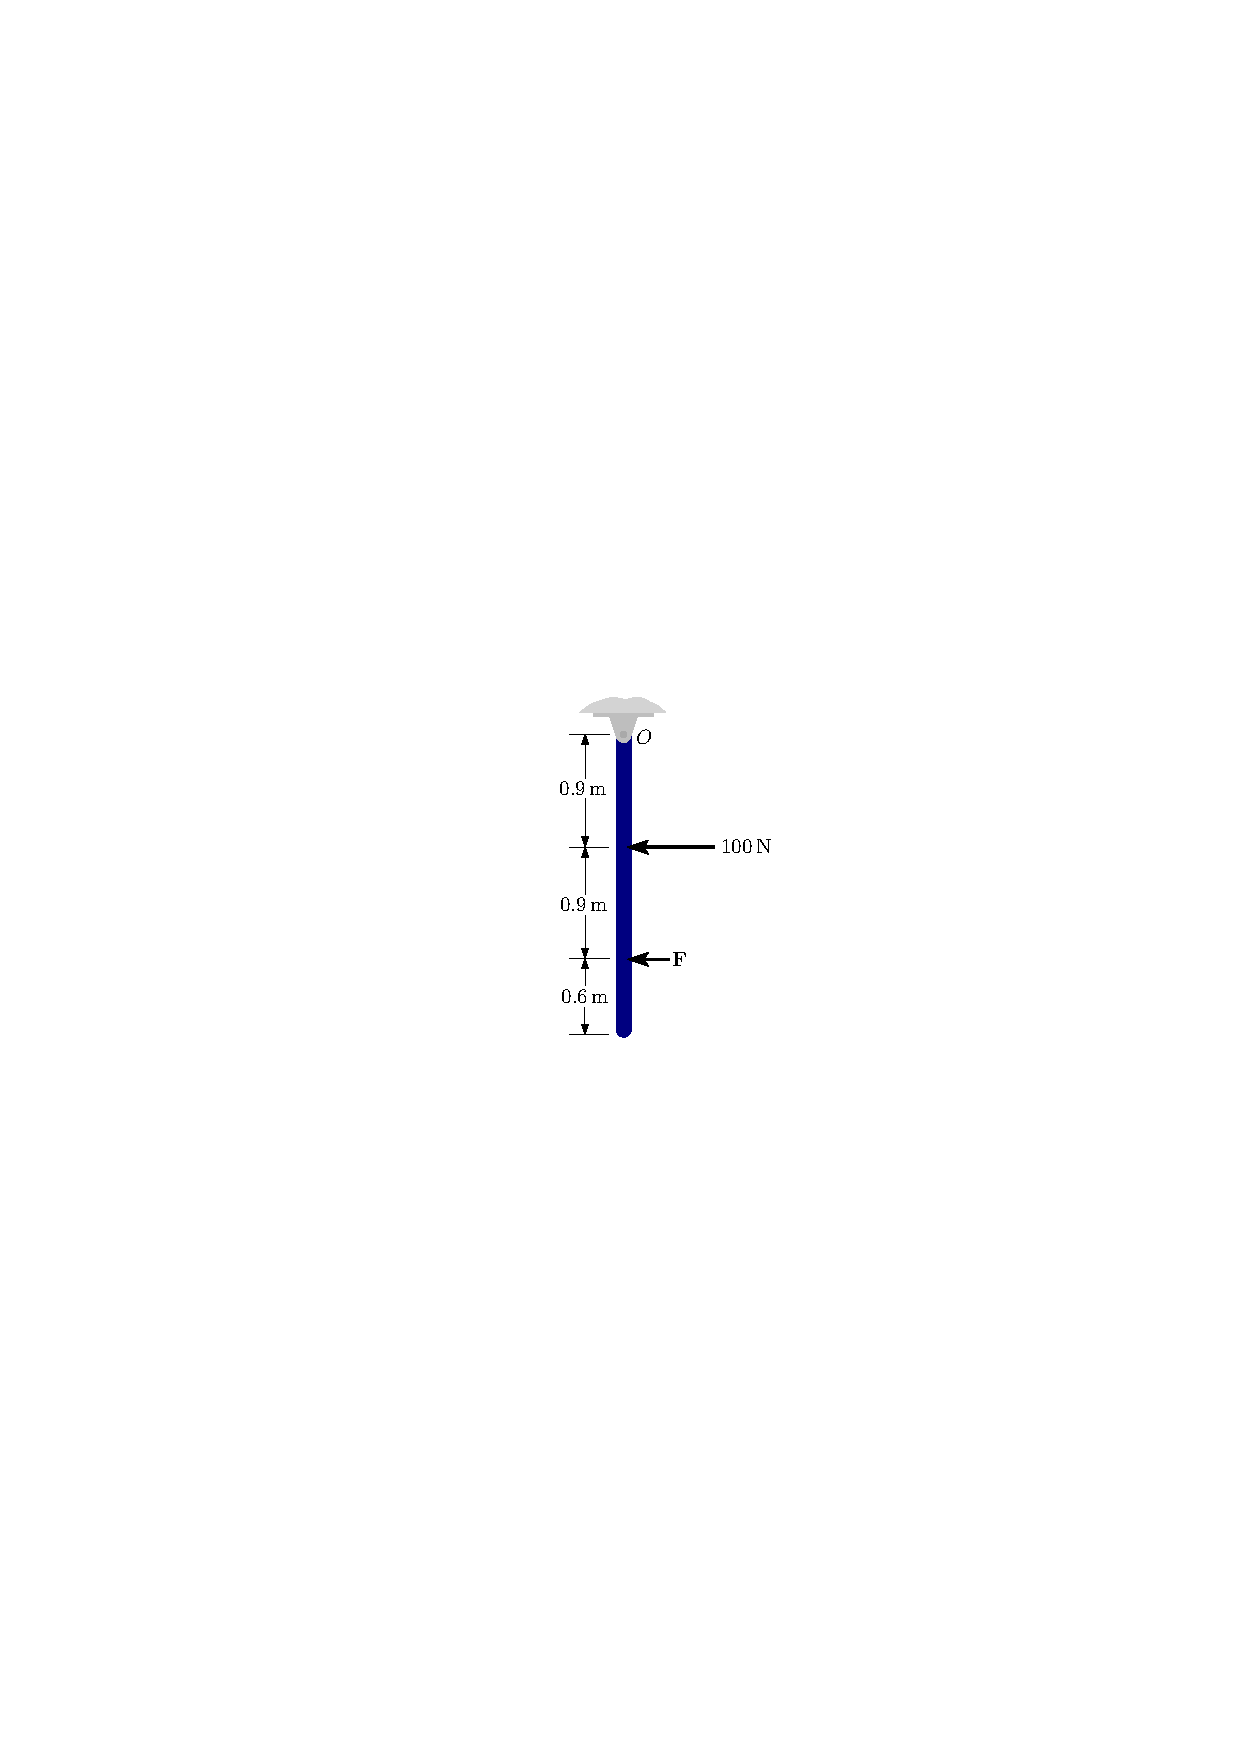
\includegraphics[scale=1.3]{../../images/draw_9}
	\end{flushright}
\end{minipage}

